% --------------------------------------------------------------
% This is all preamble stuff that you don't have to worry about.
% Head down to where it says "Start here"
% --------------------------------------------------------------
 
\documentclass[12pt]{article}
 
\usepackage{float} 
\usepackage[margin=1in]{geometry} 
\usepackage{amsmath,amsthm,amssymb}
\usepackage{listings}
\usepackage{enumitem}   
\usepackage{graphicx}
\graphicspath{ {./images/} }

\lstset{
   basicstyle=\fontsize{8}{9}\selectfont\ttfamily
}
 
\begin{document}
 
% --------------------------------------------------------------
%                         Start here
% --------------------------------------------------------------
 
%\renewcommand{\qedsymbol}{\filledbox}
 
\title{Homework 7}%replace X with the appropriate number
\author{Hai Nguyen \& Huan Nguyen\\ %replace with your name
STAT760 - Statistical Learning} %if necessary, replace with your course title
\maketitle
\textbf{Problem 1}
\begin{itemize}
    \item Train a two-layer neural network for predicting lpsa.
    \item Train the network using weight decay.
    Helper function:
    \begin{lstlisting}
function g = sigmoid(z)
g = 1./(1+exp(-z));
end
    \end{lstlisting}
    Source code (Matlab) for both cases:
    \begin{lstlisting}
clc
clear all
close all

% Import data
M = importdata("prostate.data");
N_sample = length(M);

% Exclude the first row (labels only)
for i = 2 : N_sample - 1
    temp = cell2mat(M(i, :));
    temp = strsplit(temp);
    
    % Exclude index column (column 1), True/False column (last column)
    if i == 2
        data = str2double(temp(1, 2:end-1));  
    else
        data = [data; str2double(temp(1, 2:end-1))];
    end
end

%% Train a two-layer neural network for predicting lpsa (with and without weight decay)
X = data(:, 1:end-1);

input_layer_size  = 8;
hidden_layer_size = 25;
output_layer_size = 1;

% Learning rate
lr0 = 0.1;
decay_rate = 0.95;

% 10-fold cross validation
totalSample = size(X, 1);
k_fold = 10;
test_data_size = ceil(totalSample/k_fold);

N_epoch = 1000;

% Weight decay constant
lambda = 0.05;

% Use or not use weight decay
use_weight_decay = 0;

% Randomly shuffle samples (rows)
shuffledRowIdx = randperm(totalSample);
shuffled_X = X(shuffledRowIdx, :);
shuffled_y = data(shuffledRowIdx, :);

for run = 1:k_fold
    % Get training data
    if run * test_data_size < totalSample
        
        test_index_rows = test_data_size * (run - 1)  + 1 : test_data_size * run;
        test_data_X = shuffled_X(test_index_rows, :);
        test_data_y = shuffled_y(test_index_rows, :);
        
        % Remove selected rows for test data
        copy_data_X = shuffled_X;
        copy_data_X(test_index_rows, :) = [];
        training_data_X = copy_data_X;
        
        copy_data_y = shuffled_y;
        copy_data_y(test_index_rows, :) = [];
        training_data_y = copy_data_y;
        
    else
        test_data_X = shuffled_X(test_data_size * (run - 1)  + 1 : end, :);
        test_data_y = shuffled_y(test_data_size * (run - 1)  + 1 : end, :);
        
        training_data_X = shuffled_X(1 : test_data_size * (run - 1), :);
        training_data_y = shuffled_y(1 : test_data_size * (run - 1), :);
    end

    % Normalize input
    mean_X = mean(training_data_X);
    std_X = std(training_data_X);
       
    X_norm = (training_data_X - mean_X)./std_X;

    % Scale output to [0, 1]
    min_y = min(training_data_y);
    max_y = max(training_data_y);
    t = (training_data_y - min_y)./(max_y - min_y);

    % Feedforward
    o_hat = horzcat(X_norm, ones(size(X_norm, 1), 1));

    % Initialize random weights
    W1_ = rand(input_layer_size + 1, hidden_layer_size);
    W2_ = rand(hidden_layer_size + 1, output_layer_size);

    for epoch = 1 : N_epoch
        d_W2_  = zeros(size(W2_));
        d_W1_  = zeros(size(W1_));    

        % One episode run through all sample
        for i = 1:size(training_data_X, 1)

            W2  = W2_(1 : end - 1, :);
            W1  = W1_(1 : end - 1, :);

            % Feed-forward
            out_1 = o_hat(i, :) * W1_;
            o_1 = sigmoid(out_1);
            o_1_hat = horzcat(o_1, ones(size(o_1, 1), 1));

            out_2 = o_1_hat * W2_;
            o_2 = sigmoid(out_2);

            % Back-prop
            e = o_2 - t(i);

            v2 = o_2 .* (1.-o_2);
            D2 = diag(v2);

            v1 = o_1 .* (1.-o_1);
            D1 = diag(v1);

            delta_2 = D2 * e;
            delta_1 = D1 * W2 * delta_2;

            % Decay learning rate
            lr = lr0 * decay_rate^(epoch - 1);
            
            % Weight correction
            d_W2_t = -lr * delta_2 * o_1_hat;
            d_W1_t = -lr * delta_1 * o_hat(i, :);
            
            % Add correction vector
            d_W2_ =  d_W2_ + d_W2_t';
            d_W1_ =  d_W1_ + d_W1_t';
        end

    % Update weights (use or not use weight decay)
    W2_ = W2_ + d_W2_ - lambda * use_weight_decay * lr * W2_;
    W1_ = W1_ + d_W1_ - lambda * use_weight_decay * lr * W1_;        
        
    % Testing on test-data   
    t_X_norm = (test_data_X - mean_X)./std_X;
    t_test = (test_data_y - min_y)./(max_y - min_y);        

    % Feed-forward
    t_o_hat = horzcat(t_X_norm, ones(size(t_X_norm, 1), 1));
    t_out_1 = t_o_hat * W1_;
    t_o_1 = sigmoid(t_out_1);
    t_o_1_hat = horzcat(t_o_1, ones(size(t_o_1, 1), 1));

    t_out_2 = t_o_1_hat * W2_;
    t_o_2 = sigmoid(t_out_2);

    loss(run, epoch) = 0.5 * norm(t_o_2 - t_test, 2);       
   
    end         
end

%% Plot
K = mean(loss);
plot(K);
grid on;


    \end{lstlisting}
\end{itemize}
    The error rate using k-fold cross-validation:
    \begin{itemize}
        \item Not using weight-decay:
        
        \begin{figure}[H]
        \begin{center}
          \caption{Error rate (not using weight-decay).}
          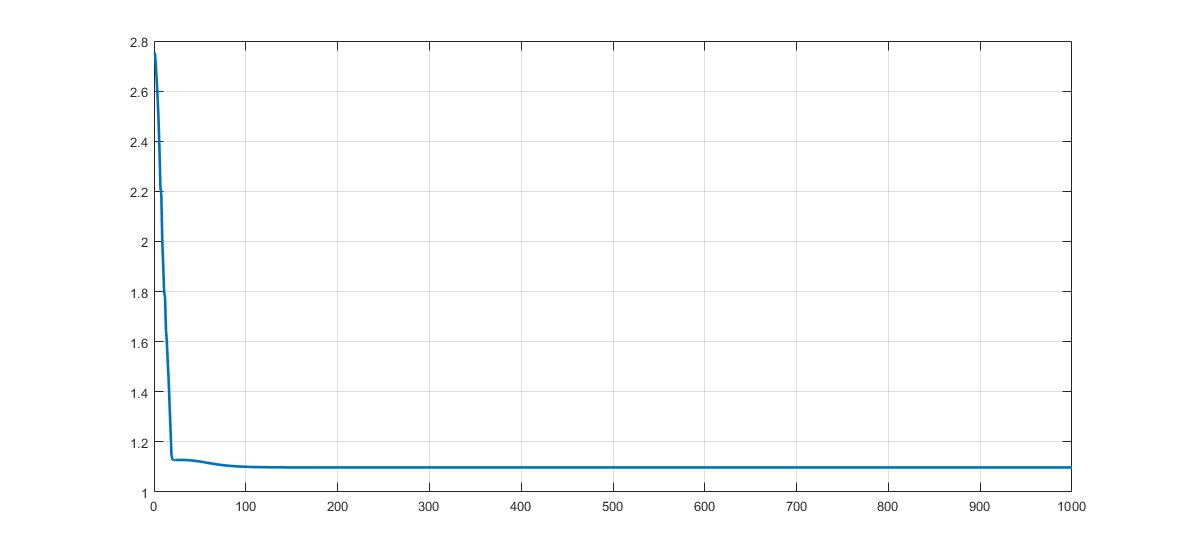
\includegraphics[width=0.75\textwidth]{images/1-1.jpg}
         \end{center}
        \end{figure}
        
        \item Using weight-decay:
        
        \begin{figure}[H]
        \begin{center}
          \caption{Error rate (using weight-decay).}
          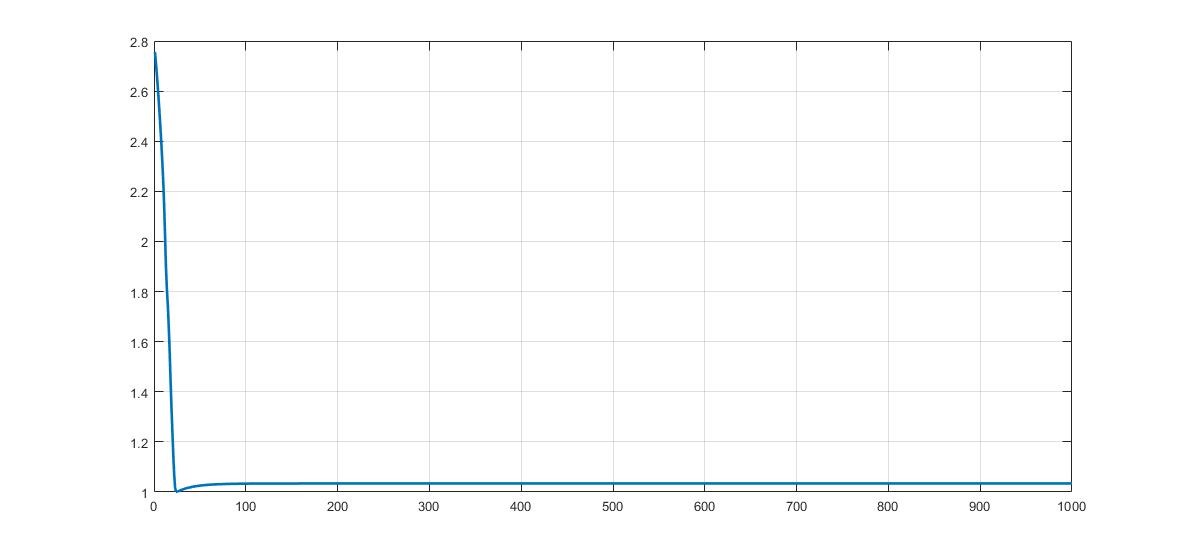
\includegraphics[width=0.75\textwidth]{images/1-2.jpg}
         \end{center}
        \end{figure}
        
    \end{itemize}
\textbf{Problem 2}
\begin{itemize}
    \item Train a two-layer neural network for predicting heart disease.
    \item Use Xavier weight initialization
    \item Train the network using dropout
\end{itemize}    
\textbf{Matlab code}
\begin{lstlisting}
close all
clear all
k = 5; % k-fold param
dropout_keeprate_layer1 = 1;
dropout_keeprate_layer2 = 1;%0.5;
learning_rate = 0.0000015;
c = 2;
N_training_max = 1000;

A = load('data_processed.txt');
N = size(A,1);
m = size(A,2) - 2; % number of predictors: ignore index and output cols
m_hidden = 10;

validate_start_idx = 0;
validate_end_idx = 0;
delta_N = round(N/k);
E_fold_CV = zeros(1, N_training_max);
E_train = zeros(k, N_training_max);
mean_ = mean(A(:, 2:m+1));
std_  = std(A(:, 2:m+1));

%% shuffle data 
A = A(randperm(N),:);

for i = 1:k
    validate_start_idx = 1 + (i-1)*delta_N;
    if (i < k)
        validate_end_idx = i*delta_N;
    else
        validate_end_idx = N;
    end
    X_CV = [(A(validate_start_idx:validate_end_idx, 2:m+1) - mean_)./std_ ...
        ones(-validate_start_idx + validate_end_idx + 1,1)];
    X_train = A(setxor(1:N, validate_start_idx:validate_end_idx), 2:m+1);
    X_train = [(X_train - mean_)./std_ ones(size(X_train,1),1)];
    delta_w1 = zeros(m+1, m_hidden);
    delta_w2 = zeros(m_hidden+1, 1);
    %% Xavier initialization
    w1 = normrnd(0, sqrt(2/(m + m_hidden)), [m+1, m_hidden]);
    w2 = normrnd(0, sqrt(2/(m_hidden + 1)), [m_hidden+1, 1]);
    %w1 = normrnd(0, 1, [m+1, m_hidden]);
    %w2 = normrnd(0, 1, [m_hidden+1, 1]);    
    
    for n = 1:N_training_max        
        dropout_mask_layer1 = (rand([1,m+1]) <= dropout_keeprate_layer1);
        dropout_mask_layer2 = (rand([1,m_hidden+1]) <= dropout_keeprate_layer2);
        for j = 1:size(X_train, 1)
            %% forward
            X = (X_train(j,:) .* dropout_mask_layer1) / dropout_keeprate_layer1;
            net1 = X * w1;
            out1_tmp = [1./(1 + exp(-c*net1)) 1];
            out1 = (out1_tmp .* dropout_mask_layer2) / dropout_keeprate_layer2;
            net2 = out1 * w2;
            out2 = 1./(1 + exp(-c*net2));
            %% backprop
            delta2 = (out2 - A(j,m+2)) .* (out2 .* (1 - out2));
            delta1 = (w2' * delta2) .* (out1 .* (1 - out1));
            delta_w2 = delta_w2 - learning_rate * 0.9^n * out1' * delta2;
            delta_w1 = delta_w1 - learning_rate * 0.9^n * X' * delta1(1:m_hidden);
            %% update training error
            E_train(i,n) = E_train(i,n) + 0.5*(out2 - A(j,m+2))^2;
        end
        E_train(i,n) = E_train(i,n)/size(X_train, 1);
        %% calculate CV error: no dropout
        w2 = w2 + delta_w2;
        w1 = w1 + delta_w1;
        net1_CV = X_CV * w1;
        out1_CV = [1./(1 + exp(-c*net1_CV)) ones(size(X_CV,1),1)];
        net2_CV = out1_CV * w2;
        out2_CV = 1./(1 + exp(-c*net2_CV));
        %error = out2_CV - A(validate_start_idx:validate_end_idx , m+2);
        out_classifier = (out2_CV > 0.5);
        E_fold_CV(n) = E_fold_CV(n) + sum(out_classifier ~= ...
        A(validate_start_idx:validate_end_idx , m+2))/(-validate_start_idx + validate_end_idx + 1);
    end
end
E_fold_CV = E_fold_CV/k;
figure
plot(E_fold_CV);
title('CV Error')
xlabel('Number of iterations')
ylabel('Error')
grid on

figure
plot(E_train');
title('Training Error')
xlabel('Number of iterations')
ylabel('Error')
grid on
\end{lstlisting}
\textbf{Error rate using k-fold cross-validation (k=5)}
\begin{itemize}
    \item Normal weight initialization, no dropout
        \begin{figure}[H]
        \begin{center}
          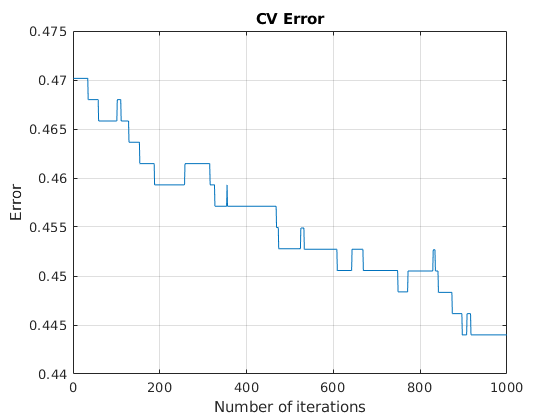
\includegraphics[width=0.75\textwidth]{images/Ex2a.png}
         \end{center}
        \end{figure}    
    \item Xavier weight initialization, no dropout
         \begin{figure}[H]
        \begin{center}
          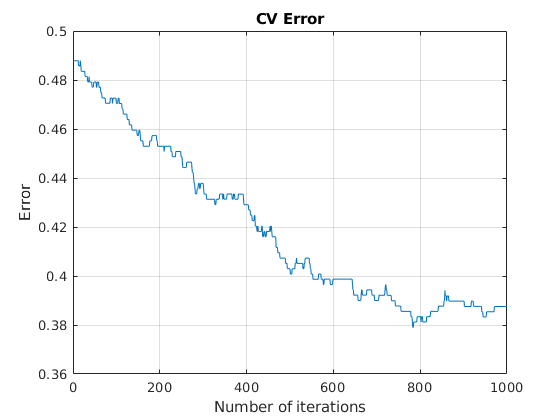
\includegraphics[width=0.75\textwidth]{images/Ex2b.png}
         \end{center}
        \end{figure}    
    \item Xavier weight initialization, using dropout at hidden layer with dropout probability 0.5
         \begin{figure}[H]
        \begin{center}
          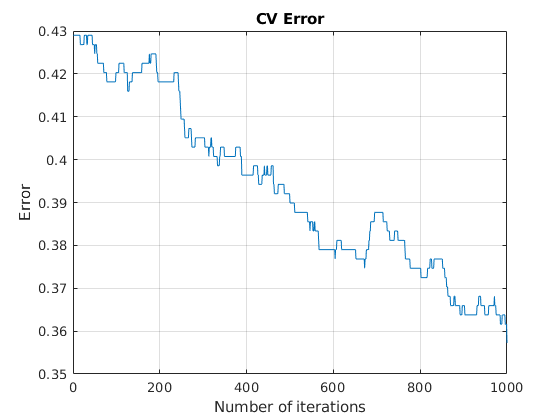
\includegraphics[width=0.75\textwidth]{images/Ex2c.png}
         \end{center}
        \end{figure}      
\end{itemize}
\end{document}